\section{Az objektumelvű programozás (OOP) alapjai}

\subsection{Bevezető}
\noindent

Az absztrakció a programozás megkerülhetetlen eleme. Amikor egy programozási nyelvet használunk, akkor rengeteg absztrakcióval találkozunk, amiket a szoftverek a hardver és a fejlesztő között felhúznak. Bizonyos szempontból még a modern szemlélettel alacsony szintűként kategorizált C nyelv is magasszintűnek tekinthető, ha azt vesszük figyelembe mennyi belső működést maszkol emberileg fogyaszthatóbb formára. A számítástechnika korai éveiben a lyukkártyás/szalagos megoldás volt a fejlesztő és a hardver közötti közös interfész. Ez rendkívül monoton, folyton ismétlődő és körülményes munkavégzést eredményezett. Az igények úgy alakították a világunkat, hogy szükség volt eszközökre amik felgyorsítják a fejlesztési folyamatot.
\bigskip

A korai absztrakciós rétegekre az Assembly nyelvek tökéletes példák. Az Assembly nagy mértékben felgyorsította a fejlesztést, emberileg olvasható utasításokat fordított át gép által értelmezhető utasításokra. Innentől nem bitsorozatokban kellett gondolkodni, hanem regiszterekben és műveletekben. Mai fejjel nem az jutna eszünkbe az Assembly-ről, hogy kifejezetten gyors fejlesztési folyamattal jár, de érdemes észben tartani, hogy a kor applikációi lényegesen egyszerűbbek voltak.

\bigskip
A következő nagy ugrásnak a magasszintű programnyelveket tekinthetjük. Korunkbeli relevanciája miatt legyen a C nyelv az alanyunk. Az Assemblyhez képest több absztrakció, ezáltal több kényelmi funkció érkezett. Nem kell regiszterekben gondolkodnunk, hanem folytonos, fentről lefele olvasható kódot, procedúrákat írunk. Definiálhatunk változókat, függvényeket, tömböket. A fejlesztési folyamat ezáltal újfent gyorsabbá válik, rövidebb időn belül komplexebb alkalmazások készültek el.

\bigskip
Ezen a ponton meg is érkezünk ahhoz a környezethez, ami az Objektumelvű Programozás igényét megszülte. Bár a procedurális nyelvek rengeteg időt spórolnak a fejlesztőknek, ezáltal komplex alkalmazások fejlesztése is lehetséges rövidebb idő alatt, a C nyelv eszközei az adatok szoros összekapcsolására (struct, union) illetve a kódszervezésre nem bizonyultak minden esetben hatékonynak vagy elégségesnek. Szemléletes példa lehet erre az alábbi kódrészlet:

//TODO

Több kérdés is felmerülhet. Elsősorban vegyük azt, hogy milyen opcióink vannak, ha VIP fiókot is implementálni szeretnénk. Legyen egy \code{int accountType} része a structnak? Nem nehéz végiggondolni, hogy ez nehézségekhez vezethet egy olyan ember számára, aki most olvassa először a kódot. Felmerülhet, hogy a szemantikai szándék egyértelműbb lenne egy \code{boolean} érték esetébenm, C-ben viszont a C99 standard-ig nem volt beépített \code{boolean} típus. Továbbá, semmi állítja meg a programozót abban, hogy tetszőleges helyen a kódon belül beállítsa a fiókok pénzösszegét tetszőleges értékűre. Ha egy ilyen jellegű hiba implementálásra kerül és átcsúszik a code review-on, akkor súlyos következményei lehetnek.

\bigskip
Az Objektumelvű programozás paradigmája ezekre, és hasonló jellegű problémákra hivatott megoldásokat biztosítani.
\newpage

\subsection{Az adattípus}
\noindent

Mielőtt belemélyedünk az paradigma központi elemeibe, nézzük meg, hogy hogyan specifikálunk egy típust. Erre azért lesz szükség, mert a típus specifikációja jól körülhatárolja majd azt, hogy milyen feladataink lesznek az objektumelvű kód tervezésekor.

\begin{figure}[H]
\centering
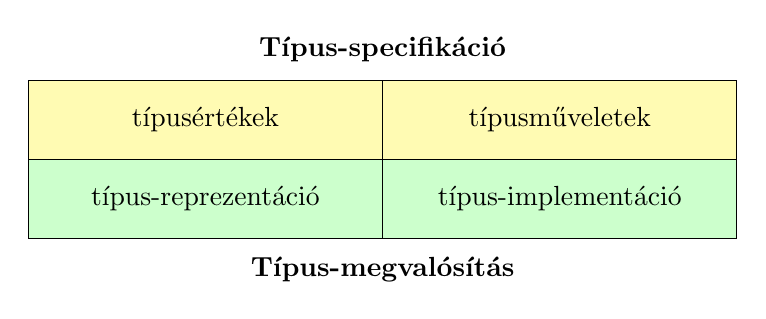
\begin{tikzpicture}
\def\cellwidth{4.5cm}
\def\cellheight{1cm}

\node at (\cellwidth, \cellheight + 0.4cm) {\textbf{Típus-specifikáció}};

\draw[fill=yellow!30] (0, 0) rectangle (\cellwidth, \cellheight);
\draw[fill=yellow!30] (\cellwidth, 0) rectangle (2*\cellwidth, \cellheight);
\draw[fill=green!20] (0, -\cellheight) rectangle (\cellwidth, 0);
\draw[fill=green!20] (\cellwidth, -\cellheight) rectangle (2*\cellwidth, 0);

\node at (0.5*\cellwidth, 0.5*\cellheight) {típusértékek};
\node at (1.5*\cellwidth, 0.5*\cellheight) {típusműveletek};
\node at (0.5*\cellwidth, -0.5*\cellheight) {típus-reprezentáció};
\node at (1.5*\cellwidth, -0.5*\cellheight) {típus-implementáció};

\node at (\cellwidth, -\cellheight - 0.4cm) {\textbf{Típus-megvalósítás}};
\end{tikzpicture}
\caption{Az adattípus felépítése}
\label{fig:adattipus}
\end{figure}

Az adattípus két komponensből áll, egy típus-specifikációból és egy típus-megvaló\-sí\-tás\-ból. A típus-specifikáció megadja az adat által felvehető értékek halmazát (\code{típusértékek}) és a típusértékekkel végezhető műveleteket (\code{típusműveletek}). A típus-megvalósítás megmutatja, hogy hogyan ábrázoljuk (\code{típus-reprezentáció}) a típusértékeket és milyen programok helyettesítsék (\code{típus-implementáció}) a műveleteket.

\bigskip
Tekintsük egy konkrét típus specifikációját, legyen ez a típus egy alma.

\begin{figure}[H]
\centering
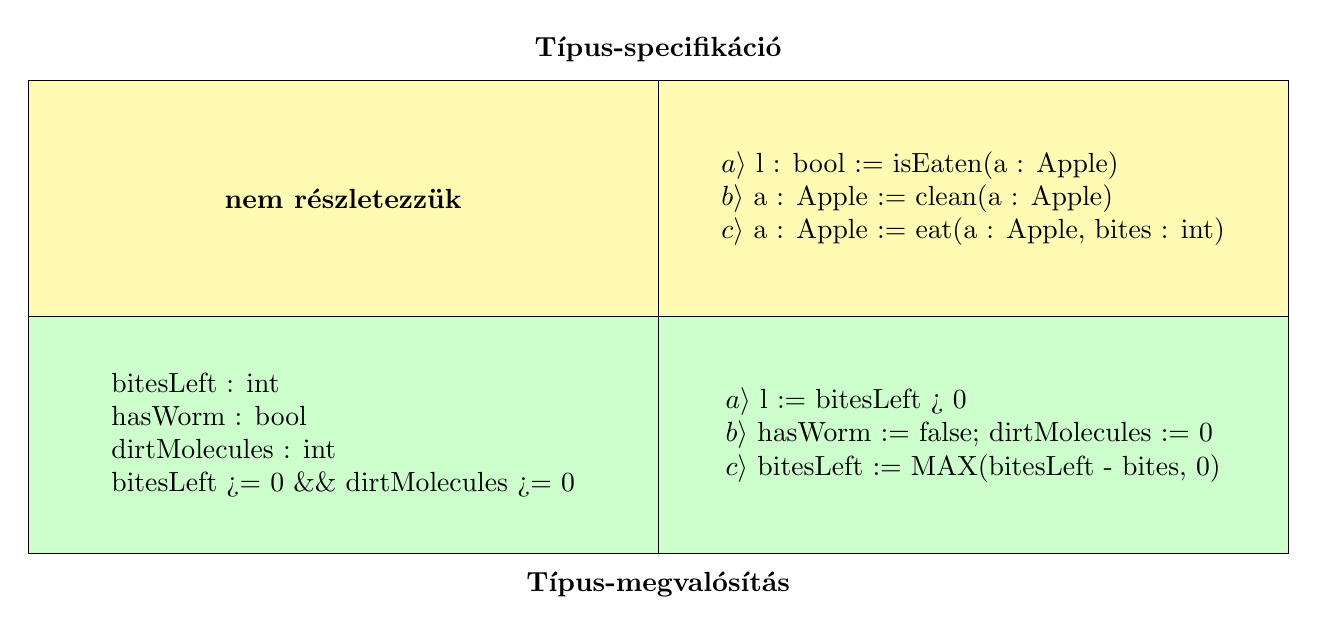
\begin{tikzpicture}
\def\cellwidth{8cm}
\def\cellheight{3cm}

\node at (\cellwidth, \cellheight + 0.4cm) {\textbf{Típus-specifikáció}};

\draw[fill=yellow!30] (0, 0) rectangle (\cellwidth, \cellheight);
\draw[fill=yellow!30] (\cellwidth, 0) rectangle (2*\cellwidth, \cellheight);
\draw[fill=green!20] (0, -\cellheight) rectangle (\cellwidth, 0);
\draw[fill=green!20] (\cellwidth, -\cellheight) rectangle (2*\cellwidth, 0);

\node[align=center] at (0.5*\cellwidth, 0.5*\cellheight) {\textbf{nem részletezzük}};
\node[align=left] at (1.5*\cellwidth, 0.5*\cellheight) {$a\rangle$ l : bool := isEaten(a : Apple)\\$b\rangle$ a : Apple := clean(a : Apple)\\$c\rangle$ a : Apple := eat(a : Apple, bites : int)};
\node[align=left] at (0.5*\cellwidth, -0.5*\cellheight) {bitesLeft : int\\hasWorm : bool\\dirtMolecules : int\\bitesLeft >= 0 \&\& dirtMolecules >= 0};
\node[align=left] at (1.5*\cellwidth, -0.5*\cellheight) {$a\rangle$ l := bitesLeft > 0\\$b\rangle$ hasWorm := false; dirtMolecules := 0\\$c\rangle$ bitesLeft := MAX(bitesLeft - bites, 0)};

\node at (\cellwidth, -\cellheight - 0.4cm) {\textbf{Típus-megvalósítás}};
\end{tikzpicture}
\caption{Az \code{Apple} adattípus}
\label{fig:apple-adattipus}
\end{figure}

Természetesen nem csak ez az egy lehetséges adattípus létezik egy alma modellezéséhez. A modell megalkotását az befolyásolja, hogy milyen műveleteket szeretnénk elvégezni egy almán. Ha például dobálni szeretnénk, akkor a tömegét is nyilván kellene tartani, és definiálni egy metódust, amely valamilyen $\theta$ szöget és valamilyen $F$ kifejtett erőt vár paraméterként.
\newpage
\subsection{Az osztály}
\noindent

Az adattípus fogalmának megismerése után ismerkedjünk meg az osztály fogalmával.

\bigskip
Az objektumelvű tervezés során osztályként adjuk meg az általunk definiált egyedi típusokat (custom type). Az osztály egy objektum szerkezetének és viselkedésének mintáját adja meg. Felsorolja az objektum \code{adattagjainak} nevét, típusát, láthatóságát, opcionálisan megadhatja az egyes adattagok típusinvariánsait, valamint megadja az objektumra meghív\-ható \code{metódusokat} névvel, paraméterekkel, visszatérési típussal, metódustesttel és látható\-ság\-gal ellátva.

\paragraph{Láthatóság:}
Az egyes adattagok és metódusok láthatósága azt mondja meg, hogy az adott objektum adattagját és metódusát milyen helyekről tudjuk elérni. A láthatóság megvalósítása eltér az objektumelvű nyelvek között.

\bigskip
Pythonból (és a legtöbb scriptnyelvből) ez a nyelvi elem például hiányzik, ezt konvenció szerint alsóvonásokkal pótolhatják a fejlesztők, azonban ezt a Python interpreter nem tartatja be szigorúan, kizárólag a fejlesztők egymás közötti kommunikációját szolgálja. Ezzel szemben Java-ban 4 láthatósági beállítás van (access modifier), C\#-ban 6-ot különböztetünk meg, ezek közül 3-at fogunk használni a félév során:

\paragraph{Public:}
Bárhonnan elérhető adattag és metódus. Jele: +.
\paragraph{Private:}
Csak osztályon belül elérhető adattag és metódus. Jele: -.
\paragraph{Protected:}
Csak osztályon belül, és leszármazottain (lásd: Öröklődés) belül elérhető adattag és metódus. Jele: \#.
\subsection{Az objektum}
\noindent

Az Objektumelvű programozás központi eleme az objektum. Objektumnak a feladat azt az önálló egyedként azonosított részét nevezzük, amely magába foglalja az általa ellátott részfeladat megoldásáért felelős adatokat és műveleteket. Az objektumokra létrehozásuk után közvetett módon, egy változóval tudunk hivatkozni. Ez a változó tartalmazza a program futása közben az objektum által használt memóriaterület címét.

\begin{csharpblock}
Object obj1 = new Object();
\end{csharpblock}

A fenti kódrészletben a \code{new} kulcsszót használva hozzuk létre az objektumot, az \code{Object()} adja meg hogy milyen objektumot hozunk létre (jelen esetben ez az \code{Object} ősosztály), az \code{obj1} pedig a fent említett változó.


\subsection{Speciális osztályok}
\subsubsection{Felsoroló (Enum)}
\subsubsection{Interfész (Interface)}
\subsubsection{Absztrakt osztály (Abstract class)}

\input{chapters/02-oop-basics/class-relationships}
